\documentclass[twoside, a4paper]{article}
\usepackage[english]{babel}
\usepackage{a4wide}

% Fonts
\usepackage[sc]{mathpazo}
\usepackage[T1]{fontenc}
\linespread{1.05}
\usepackage{microtype}
\usepackage{lettrine}

% References
\usepackage{varioref}
\usepackage{hyperref}
\usepackage{cleveref}

% Document layout
% \usepackage[hmarginratio=1:1,top=32mm,columnsep=20pt]{geometry}
\usepackage{multicol}
\usepackage{paralist}

% Floats
\usepackage{float}

%Plaatjes
\usepackage{graphicx}
\usepackage[hang, small,labelfont=bf,up,textfont=it,up]{caption}
\usepackage{subcaption}

% Tables
\usepackage{booktabs}

% Custom section headers
\usepackage{titlesec}
\renewcommand\thesection{\Roman{section}}
\renewcommand\thesubsection{\Roman{subsection}}
\titleformat{\section}[block]{\large\scshape\centering}{\thesection.}{1em}{}
\titleformat{\subsection}[block]{\large}{\thesubsection.}{1em}{}


%Wiskunde
\usepackage{siunitx}
\usepackage{mathtools}
\usepackage{amsmath}
\usepackage{amsfonts}
\usepackage{amssymb}

% References
\usepackage[backend=bibtex]{biblatex}
\usepackage{csquotes}
\bibliography{biblio}

% Temp
\usepackage{todonotes}

% Math commands
\newcommand{\normal}[2]{\ensuremath{\mathcal{N}\left(#1,\, #2\right)}}
\renewcommand{\vec}[1]{\ensuremath{\mathbf{#1}}}

% Other commands
\renewcommand{\t}[1]{\texttt{#1}}

\title{Modelling and Simulation\\Practical Assignment I: The Chirikov map}
\author{Rick van Veen (s1883933) \and Laura Baakman (s1869140)}

\begin{document}

\maketitle

% \todo[inline]{Use compactitem environment for lists}

\begin{multicols}{2}

\section{Introduction}
%!TEX root = practicum2.tex
\todo[inline]{Tijd over: Blaat over toepassing van model}
\noindent This paper first presents and then discusses a percolation model. \Cref{s:method} presents the model we used and an implementation in pseudo code. In \cref{s:experiment} we discuss some of the experiments we have performed with the model and their results. \Cref{s:conclusion} presents a summary of the findings of our experiment. 


	
\section{Method}
%!TEX root = practicum2.tex
\Cref{alg:percolation} presents our iterative growth process, the method \FuncSty{percolation} expects three arguments \t{mask}, \t{probability} and . Given the size parameter \t{N}, the grid used for the percolation is $(2N + 1) \times (2N + 1)$, this causes the grid to have an uneven number of rows and columns. Consequently the grids center is always clearly defined as $(N + 1, N + 1)$. The parameter $p \in [0, 1]$ is the probability that a given site in the cluster becomes occupied. The \t{mask} is a binary matrix with $r$ rows and $c$ columns that determines the used connectivity. Until \cref{ss:exp:connectivity} we only consider four-connected clusters, for which the mask presented in \cref{fig:exp:connectivity:fourMask} is used.\\

\begin{figure}
	\centering
	\begin{subfigure}{0.45\columnwidth}
		\centering
		
\includegraphics[width=0.8\textwidth]{./img/exp_mask_four.jpg}
		\caption{4-connectivity}
		\label{fig:exp:connectivity:fourMask}
	\end{subfigure}
	\begin{subfigure}{0.45\columnwidth}
		\centering
		
\includegraphics[width=0.8\textwidth]{./img/exp_mask_eight.jpg}
		\caption{8-connectivity}
		\label{fig:exp:connectivity:eightMask}
	\end{subfigure}	
	\caption{Connectivity masks for \subref{fig:exp:connectivity:fourMask} four-connectivity and \subref{fig:exp:connectivity:eightMask} eight-connectivity. The red squares are considered neighbors of the blue center square.}
	\label{fig:exp:connectivity}
\end{figure}

\begin{algorithm}[t]
	\setstretch{1.2}
	\SetAlgoShortEnd
	\DontPrintSemicolon
	\SetKwInOut{Input}{input}\SetKwInOut{Output}{output}
	\Input{$N$ size\\
		$p$ probability\\
		$mask$ $r \times c$ binary matrix\\
		$seed$ for the random generator}
	\Output{$grid$ $(2N + 1) \times (2N + 1)$ matrix}
	\BlankLine

	$center$ := ($N + 1$, $N + 1$)\; 

	\FuncSty{push($queue$, $center$)}\; 
	$grid$ := \FuncSty{initGrid($N$, $N$)}\; 
	$probabilities$ := \FuncSty{rand($N$, $N$)}\; 

	\While{not \FuncSty{isEmpty($queue$)}}{
		$site$ = \FuncSty{pop($queue$)}\; 
		\nosemic $sites$ = \FuncSty{grow}($grid$, $site$, $mask$, $p$,\;
		\pushline\dosemic $probabilities$)\; 
		\popline \If{anyOnBorder(sites)}{
			\KwSty{break}
		} 
		\FuncSty{push($queue$, $sites$)}\; 
	}\; 
	\caption{\FuncSty{percolation}$(mask, N, p)$\label{alg:percolation}}
\end{algorithm}

% Initialisation
Initially the only site we have to consider is the center site, which is consequently the only site in the queue at the first iteration. The matrix \t{probabilities} stores for each site the probability that it may grow, it is generated by sampling an uniform distribution with the range $[0,1]$ $(2N + 1)^2$ times. 

% Iteratie
Each iteration we pop the next \t{site} from the queue. We grow this point, using the function \t{grow}. This method considers all neighbors that are connected to \t{site} as determined by the \t{mask}. For each of these neighbours we retrieve the value $z$ from \t{probabilities}. If $z \leq p$ we mark the neighbor site as occupied, otherwise it is marked empty. The method \t{grow} returns the newly occupied neighboring sites, which are then added to the queue, so they can be processed by the \t{grow} process in a later iteration.

% Stop conditions
The growth of the clusters stops when the queue is empty and it thus cannot grow anymore or if it has reached one of the borders of the grid. In the first case the cluster is finite, which means that all neighboring sites of the cluster, according to the connectivity defined by the \t{mask}, are marked as empty. In \cref{alg:percolation} we test for this condition via the guard of the loop; if the queue is empty there are no more neighbors to consider, consequently the cluster must be finite. 

\begin{figure}[t!]
	\centering	
	\begin{subfigure}{\columnwidth}
		\centering
		
\includegraphics[width=\textwidth, height=0.225\textheight, keepaspectratio=true]{./img/fancy_cluster_N20_p3_rng_8}
		\caption{$N = 20$ and $p = 0.3$}
		\label{fig:method:fin_inf:finiteSmall}
	\end{subfigure}

	\begin{subfigure}{\columnwidth}
		\centering
		
\includegraphics[width=\textwidth, height=0.225\textheight, keepaspectratio=true]{./img/fancy_cluster_N20_p5_rng_8}
		\caption{$N = 20$ and $p = 0.5$}
		\label{fig:method:fin_inf:finiteLarge}
	\end{subfigure}

	\begin{subfigure}{\columnwidth}
		\centering
		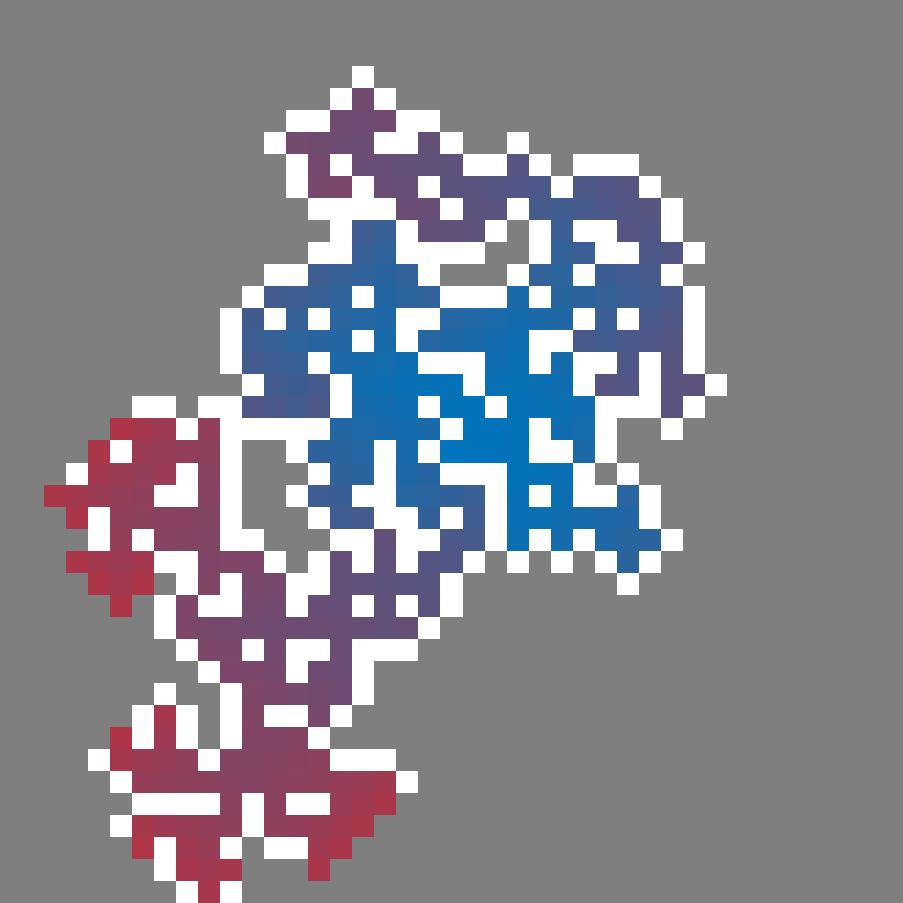
\includegraphics[width=\textwidth, height=0.225\textheight, keepaspectratio=true]{./img/fancy_cluster_N20_p6_rng_5}
		\caption{$N = 20$ and $p = 0.6$}
		\label{fig:method:fin_inf:infinite}
	\end{subfigure}	
	\caption{Examples of \subref{fig:method:fin_inf:finiteSmall} a small finite cluster, \subref{fig:method:fin_inf:finiteLarge} a larger finite cluster and \subref{fig:method:fin_inf:infinite} a percolating cluster using four-connected neighbours. The colours of the elements in the cluster indicate when that point was added to the cluster, the `colder' the color the earlier in the percolation it was added to the cluster. White cells are empty and gray cells are undetermined. }
	\label{fig:method:fin_inf}
\end{figure}


A percolating cluster is a cluster that has reached the border of the grid, i.e. if there is an occupied site with row or column number $1$ or $2N + 1$. We test for this condition with the method \t{anyOnBorder} which is called before adding newly occupied sites to the queue.\\
% Which has a consequence...

\Cref{fig:method:fin_inf} presents three clusters grown with \cref{alg:percolation}. We can clearly see that the finite clusters are completely surrounded by a white border, which indicates that these sites are empty and processed. \Cref{fig:method:fin_inf:infinite} shows a percolating cluster, which has stopped growing due to a site in the lower left corner.
\todo[inline]{Anders formuleren!!}
Another indication of the percolating nature of the cluster is the fact that there are occupied sites that can still grow, as indicated by their empty, i.e. grey, neighbours.

	

\section{Experiments}
%!TEX root = practicum1.tex

\subsection{Fixed $K$}


\begin{figure}
	\centering
	% \x/\picname in {4/pic1.png,8/pic2.png,15/pic3.png,16/pic4.png}
	\foreach \dim/\x/\p in {0/0.500/0.500, 1/0.1576131/0.9705928, 2/0.1269868/0.9133759}
	{ 
		\begin{subfigure}[t]{0.32\textwidth}
			\includegraphics[width=\textwidth]{./img/assignment_a_\dim_dim.pdf}
			\caption{$x_0=\num{\x}$, $p_0=\num{\p}$}
			\label{fig:experiment:dimension:\dim}
		\end{subfigure}
		\begin{subfigure}[t]{0.32\textwidth}
			\includegraphics[width=\textwidth]{./img/assignment_a_\dim_dim_progression_p.pdf}
			\caption{Progression of $p$ in \subref{fig:experiment:dimension:\dim}}
			\label{fig:experiment:dimension:\dim:x}
		\end{subfigure}		
		\begin{subfigure}[t]{0.32\textwidth}
			\includegraphics[width=\textwidth]{./img/assignment_a_\dim_dim_progression_x.pdf}
			\caption{Progression of $x$}
			\label{fig:experiment:dimension:\dim:p}
		\end{subfigure}		
	}
	\caption{}
	\label{fig:experiment:dimension}
\end{figure}

\subsection{Variable $K$}	

\section{Conclusion}
%!TEX root = practicum1.tex

In our discussion of the Chirikov map we have seen some simularities with the logistic map. As is the logistic map, the Chirikov is non-linear i.e. it produces output not necesary proportional to the input. Both maps are also driven by a variables which determines the amount of chaos in the system, and depend on this variable. Meaning that lower values will result in no chaotic behaviour at all. As shown for the Chirikov map in \cref{fig:experiment:fancy_k} where for low $K$ values the $x_n$ and $p_n$ values stay approximately in the same area, when $K$ is small. An important difference is that the Chirikov map produces two dimensional output, which also depend on each other (see \eqref{eq:chirikov}, where the logistic map only produces one. \todo[inline]{And some other things.. period doubling, stable points?}

\printbibliography

\end{multicols}
\end{document}